\chapter{Automatización}

\todo{explicar la forma de dividir los plugins y su conveniencia frente a otras}
\todo{comprobar que en todos sitios figura protégé en lugar de otras locuciones.}

La ontología mostrada se ha desarrollado utilizando el framework Protégé\cite{Stanford-Protégé:WEB}. Protégé\todo{Instalar Protégé en /opt - mirar LHS Linux Hierarchy system en google} es un editor de ontologías libre, con una filosofía ´´open source'' que además soporta varios formatos, entre los que destaca OWL\cite{W3C-OWL:WEB}. Protégé ha sido desarrollado por el centro de investigación informática y biomédica\cite{Stanford-BMIR:WEB} de la Escuela Universitaria de Medicina de la universidad de  Standford\cite{Stanford-MED:WEB}, con la colaboración de DARPA, eBay, National Cancer Institute, National Institute of Standards and Technology, National Library of Medicine y National Science Foundation, entre otros.

Gracias al formato OWL soportado por Protégé, a su filosofía de software libre, y a los apoyos recibidos por parte de diversas instituciones como las arriba mencionadas, existen multitud de herramientas disponibles para trabajar demanera automática con las ontologías creadas por Protégé, ya sea en forma de plug-in's o en forma de herramientas que trabajan directamente sobre la ontología en formato OWL. Además, en versiones de Protégé posteriores a la 3.x, es posible exportar directamente desde la herramienta, métodos en lenguaje java (gracias a OWL2API) que permiten trabajar con esa ontología desde un programa java.

Gracias al uso de un lenguaje estructurado como OWL-DL, es posible la utilización de herramientas automáticas que facilitan la presentación y el manejo de la información, de modo que pueda resultar más usable para los diversos actores que utilizarán la ontología: profesores, alumnos, administraciones públicas y privadas... Estas personas y/o entidades podrán trabajar con documentos html, grafos y diagramas más comprensibles que la mera expresión de la ontología en sintaxis manchester (o cualquier otra sintaxis a la que quisiéramos exportar la información). Además, dado que las ontologías son en sí mismas un modelo de datos, también es posible generar a partir de ella diferentes modelos de datos, como el modelo UML o el relacional.

Por último, gracias al carácter completo y decidible del lenguaje utilizado, resulta posible (y muy útil) utilizar herramientas capaces de llevar a cabo labores de razonamiento sobre la ontología creada, de modo que nos sea posible descubrir errores o inconsistencias en su diseño (insatisfactibilidad de un concepto, subsunción de conceptos, \ldots) y en las instancias del mismo (consistencia de ABox y TBox). 

Es por ello que se ha optado por realizar una enumeración de las diferentes herramientas que es posible utilizar, atendiendo al tipo de tarea que dicha herramienta automatiza. Así tendremos herramientas que llevan a cabo algún tipo de razonamiento sobre la ontología, herramientas que permiten la transformación de la ontología en diversos tipos de datos para ampliar su aplicabilidad, editores que permiten manipular la ontología y las diversas instancias creadas sobre ella, visores que nos presentan la información contenida en la ontología en las más diversas formas, y otras herramientas que automatizan las más diversas tareas, como veremos más adelante.

\section{Razonadores}

\subsection{FaCT++} Es una mejora sobre el anterior razonador FaCT, que hace uso de los mismos algoritmos que éste, pero con una implementación mejorada. Además está creado utilizando el lenguaje C++ lo que ha incrementado su eficacia y su portabilidad. Ha sido desarrollado por la Universidad de Manchester y se instala de forma predeterminada junto con Protégé.

http://protegewiki.stanford.edu/wiki/RacerProTG

\subsection{HermiT} es un razonador para ontologías OWL. HermiT es capaz de determinar si una ontología es o no consistente, identifica relaciones del tipo "es un" y más. Hace uso de un nuevo algoritmo que lo hace más eficaz que cualquier otro utilizado anteriormente, y cumple con los estándares OWL2. La versión utilizada es la 1.3.6. Es un razonador de código abierto bajo licencia LGPL.

\subsection{RacerPro} RacerPro\footnote{http://protegewiki.stanford.edu/wiki/RacerProTG} Es el nombre comercial de un razonador para OWL. Existe un plugin para Protégé llamado RacerProTG que trabaja de forma automática con la última versión disponible del razonador RacerPro (existe una licencia gratuita y permanente para el uso del plugin junto con Protégé). 



\subsection{Editores}

\subsubsection{ACE View} ACE View\footnote{http://attempto.ifi.uzh.ch/aceview/} es un editor de reglas y ontologías que mediante el uso de Attempto Controlled English\footnote{Attempto Project: http://attempto.ifi.uzh.ch/site/} permite crear, ver, editar, e interrogar ontologías OWL y conjuntos de reglas SWRL. Permite obviar los detalles de OWL y SWRL, ya que el usuario trabaja directamente en ACE, e incluso permite su utilización simultánea con otros editores que trabajen sobre OWL.

Permite obtener de manera rápida una lectura en lenguaje seminatural (inglés en este caso). Existe el problema de que el visor no es capaz de interpretar reglas inferidas por el razonador, sino únicamente aquellas definidas manualmente. De igual modo, no le es posible trabajar con ontologías importadas, lo cual limita su uso (para este caso en particular) a una lectura de la traducción de la ontología a ACE. Si fuese preciso explotar al máximo esta herramienta, podríamos entonces exportar la ontología a una única fuente autocontenida.

A modo de ejemplo, se muestra una parte de la ontología:

{\ttfamily\footnotesize
\begin{verbatim}
		Everything that is AS-formaParteDe-MAed by something is a Materia.
		Everything that MA-seImparteMediante-MEs something is a Materia.
		/* MOS: OG-Descripcion Range: string */
		Everything that UT-contiene-MAs something is an Ubicacion-temporal.
		Everything that is UT-contiene-ASMAed by something is something that is an Asignatura or that is a Materia.
		If X AS-tieneComoRequisito-ASes Y then Y AS-esRequisitoPara-ASes X. If X AS-esRequisitoPara-ASes Y then Y AS-tieneComoRequisito-ASes X.
		If X UT-contiene-ASes Y then X UT-contiene-ASMAs Y.
		Everything AS-ubicada-UTs at most 1 thing.
		Everything that is UT-contiene-ASed by something is an Asignatura.
		If X MA-constaDe-ASes something that AS-ubicada-UTs Y then X MA-ubicada-UTs Y.
		Everything that MV-esUtilizadoEn-MAs something is a Me-Evaluacion.
		Everything is MA-constaDe-ASed by at most 1 thing.
		Everything that is MA-otorgaCompetenciasGenerales-CGed by something is a Competencia-General.
\end{verbatim}
}

\subsubsection{ChangeView} Este\footnote{http://code.google.com/p/co-ode-owl-plugins/wiki/ChangeView} Plugin resulta muy útil durante el desarrollo de la ontología, ya que nos permite tener un control de cambios realizados desde la apertura de la ontología. El listado de cambios sigue un orden cronológico, por lo que siempre sabemos cuál a sido el último cambio realizado en la ontología, lo que nos permite desahcer los cambios deseados.

\begin{center}
		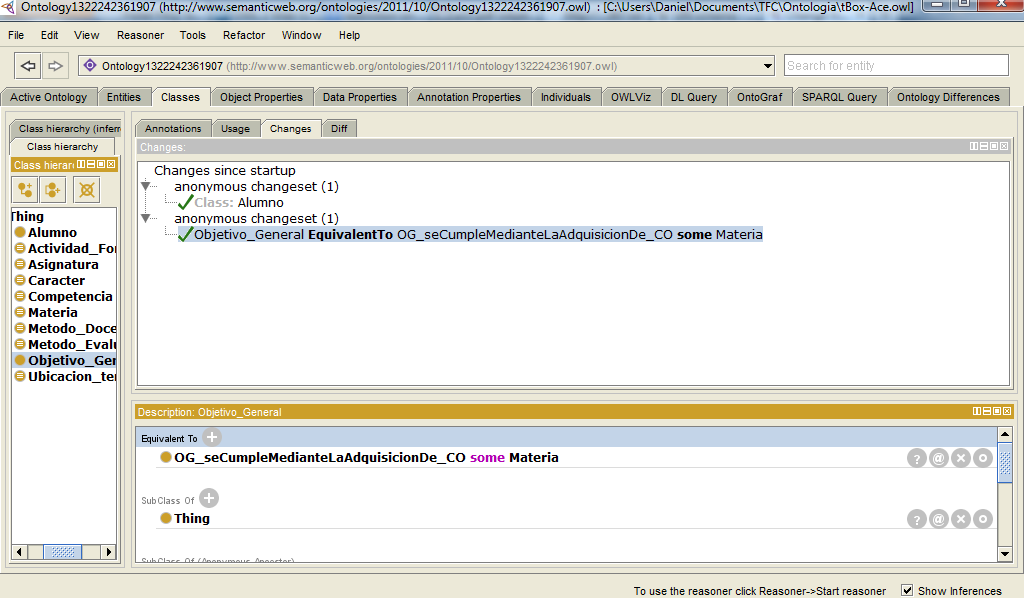
\includegraphics[width=1.00\textwidth]{Imagenes/Herramientas-changeview.png}
\end{center}

\subsubsection{HypergraphDB} es un software que permite la colaboración de un equipo y realizar el control de versiones desde dentro de Protégé. Este plugin ha sido desarrollado por el condado de Miami-Dade, pero la página del proyecto \footnote{http://sharegov.org/\#\%21../protegehgdb/owltools.html} permanece caída en el día de la fecha y no se han encontrado en internet fuentes adicionales a esta para la obtención del plugin. No obstante, el proyecto HypergraphDB continúa, y desde su página \footnote{http://www.hypergraphdb.org/index} podemos descargar la última versión del software e instrucciones sobre su uso, con lo que resulta relativamente sencillo contruir un plugin que, haciendo uso de la OWL API 2.2\footnote{http://owlapi.sourceforge.net/}.

\todo{Comprueba que la página sigue caída.}

\subsection{Visores}

Los visores nos permiten visualizar la información de manera más sencilla, de modo que aumenta la comprensión de la información y la claridad de la misma. De este modo resulta más fluido el intercambio de información entre los usuarios de la ontología.

\subsubsection{CloudViews}. Este plugin\footnote{http://code.google.com/p/co-ode-owl-plugins/wiki/CloudViews} nos permite ver la ontología como una nube de tags. Podemos selecionar ver las clases, propiedades e individuos y representarlos en una nube de tags. Estos tags pueden ordenar los conceptos en función del uso, de su profundidad y en función otras características.

Permite exportar los resultados a formato html que luego pueden visualizarse en un navegador web y que al pinchar sobre ellos nos permitiría abrir en una nueva página la documentación del tag.

\begin{center}
		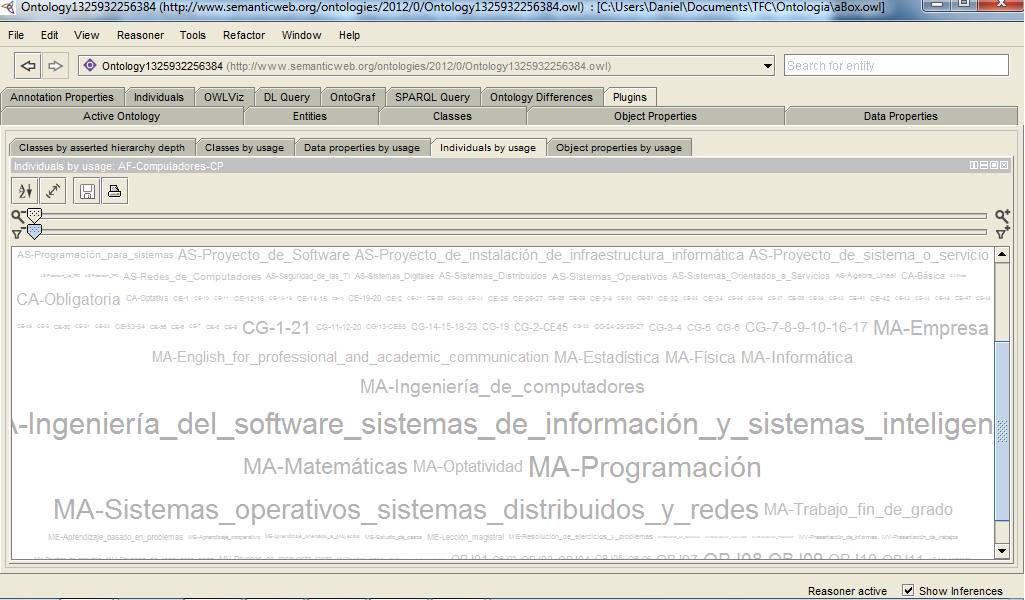
\includegraphics[width=1.00\textwidth]{Imagenes/Herramientas-cloudview.png}
\end{center}

\subsubsection{Matrix} El plugin Matrix\footnote{http://code.google.com/p/co-ode-owl-plugins/wiki/MatrixViews} nos permite tener una visión de la ontología en forma de tabla, seleccionando aquella información que de las diferentes clases, propiedades e individuos nos interesa. Incluso es posible, desde la propia tabla, incluir información en la ontología, lo que la convierte en muy útil para completar información.

\begin{center}
		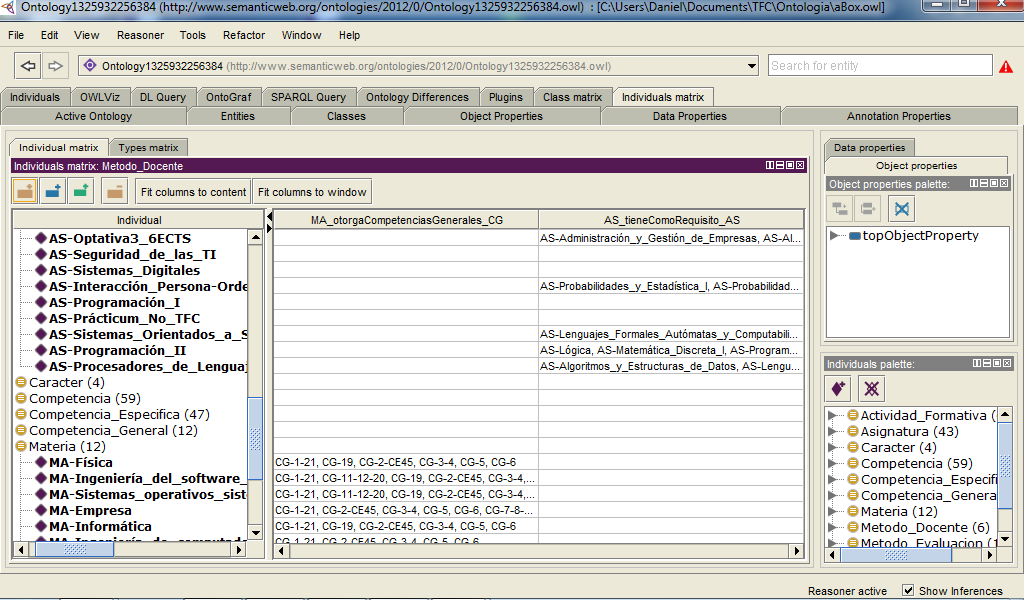
\includegraphics[width=1.00\textwidth]{Imagenes/Herramientas-matrix.png}
\end{center}
\begin{center}
		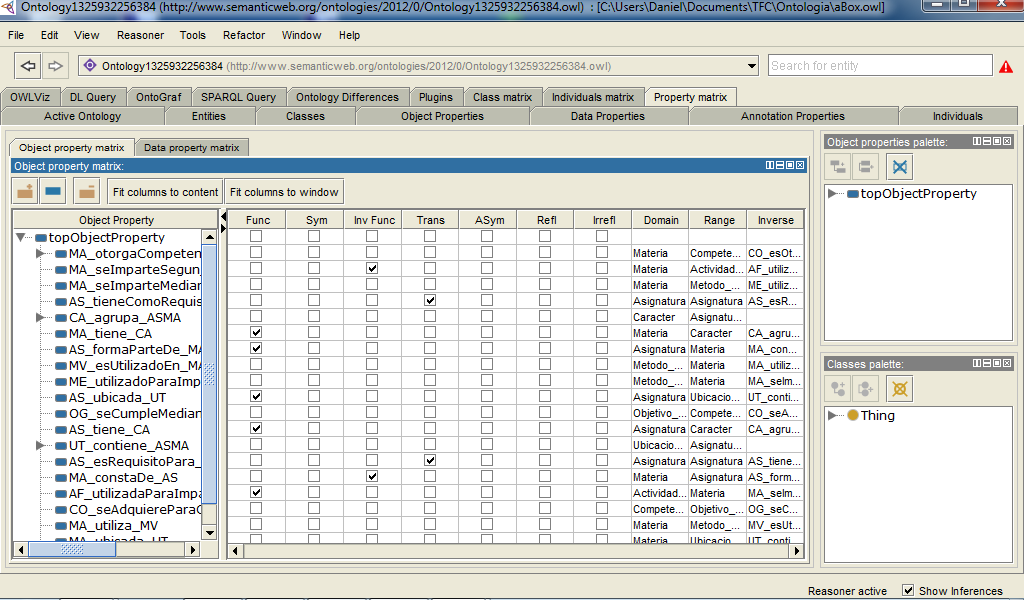
\includegraphics[width=1.00\textwidth]{Imagenes/Herramientas-matrix2.png}
\end{center}

\subsubsection{NavigOWL} NavigOWL\footnote{http://klatif.seecs.nust.edu.pk/navigowl/index.html} es una herramienta de visualización especialmente diseñada para explorar ontologías y permitir una mejor comprensión de su estructura. Los gráficos pueden mostrarse en pantalla según diferentes técnicas de modo que sea más fácil comprender la importancia de cada nodo, al aparecer este de mayor tamaño. También es posible mostrar u ocultar las etiquetas de los diferentes nodos o redistribuirlos en el lienzo. La herramienta incorpora una función de búsqueda que permite localizar en el grafo cualquier nodo de la ontología, lo que también facilita el examen de la misma.

\begin{center}
		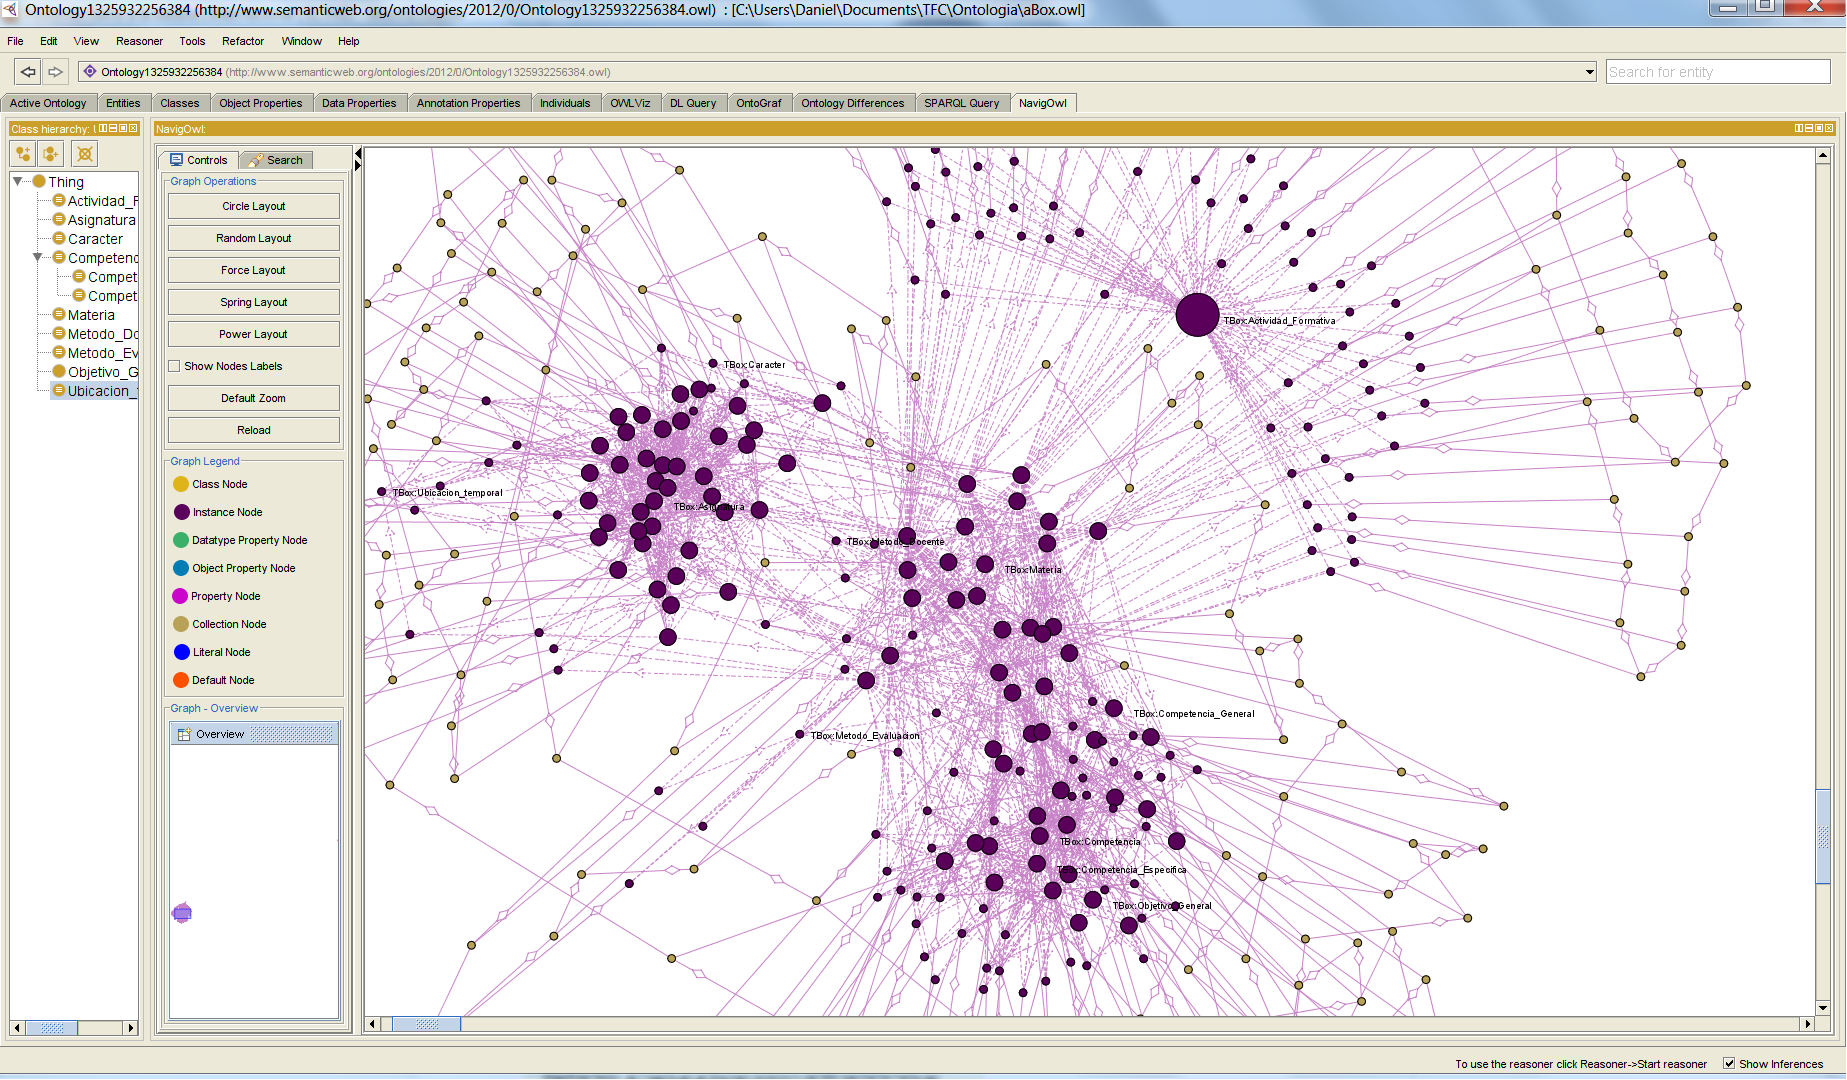
\includegraphics[width=1.00\textwidth]{Imagenes/Herramientas-NavigOwl.png}
\end{center}

\subsubsection{Ontograf} Ontograf\footnote{http://protegewiki.stanford.edu/wiki/OntoGraf} es otro visor de ontologías. A diferencia de NavigOWL, todos los nodos tienen la misma representación, sin poder establecer a priori una clasificación en función de su importancia, pero a cambio resulta mucho más ágil de manejar que NavigOWL, ya que en ontologías grandes como la nuestra, no resulta una aplicación tan pesada de mover. Se puede elegir si deseamos que nos muestre individuos o clases e incluso podemos ocultar clases o individuos que estén relacionados mediante una propiedad en particular.

Admite las relaciones de subclases, individuos, dominio y rango de las propiedades y equivalencias. También se pueden personalizar, para cada tipo de nodo, la información que queremos visualizar.

\todo{Captura realizada antes de la unión de abox y tbox}

\begin{center}
		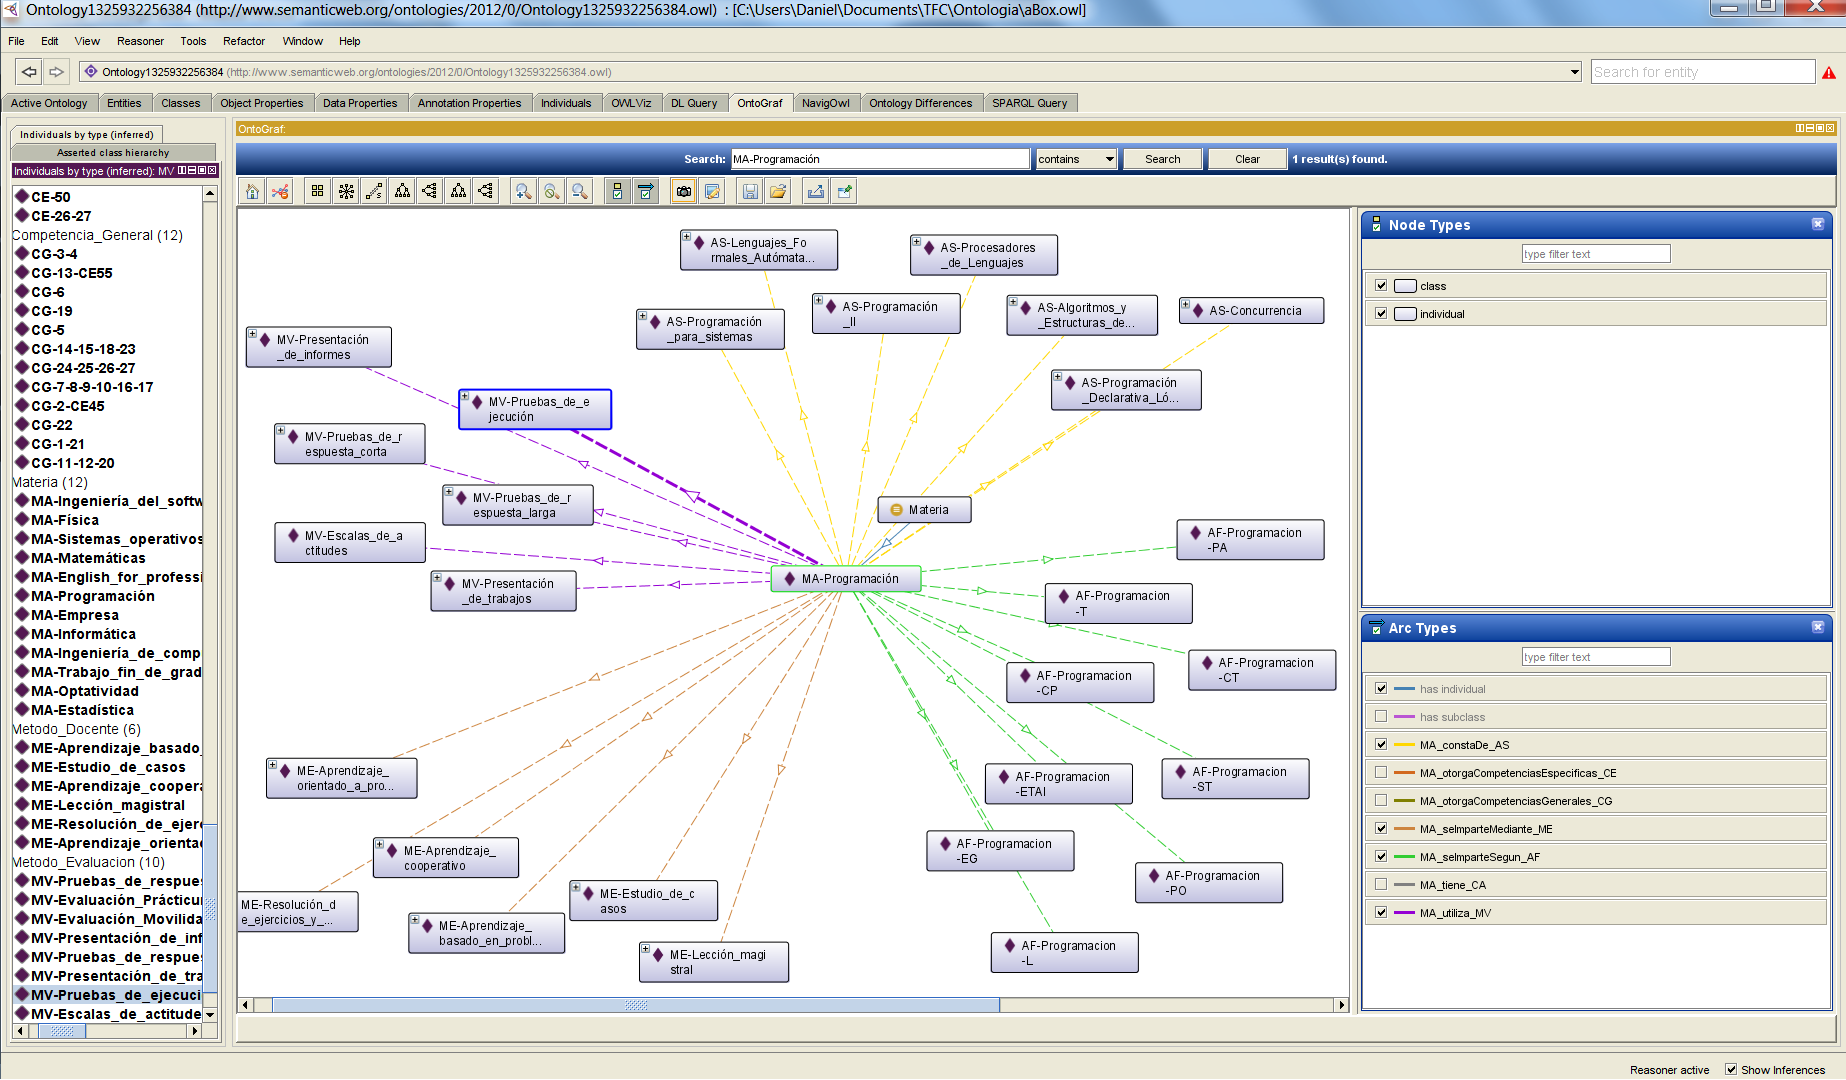
\includegraphics[width=1.00\textwidth]{Imagenes/Herramientas-OntoGraf.png}
\end{center}

\subsubsection{OWLGrEd} OWLGrEd es un editor gráfico para ontologías OWL. Permite visualizar ontologías existentes en diagramas UML y la creación y desarrollo de ontologías desde el entorno gráfico. Las ontologías creadas pueden ser exportadas a Protégé para comprobar su consistencia, realizar una clasificación, etc, o también importadas desde Protégé a la herramienta.

Es un modo de ver la estrucutra de la ontología muy rápidamente, pero cuenta con el inconveniente de que, en ontologías grandes con muchos individuos, el tiempo de carga la hacen inviable.
\todo{captura realizada antes de la unión de abox y tbox}

\begin{center}
		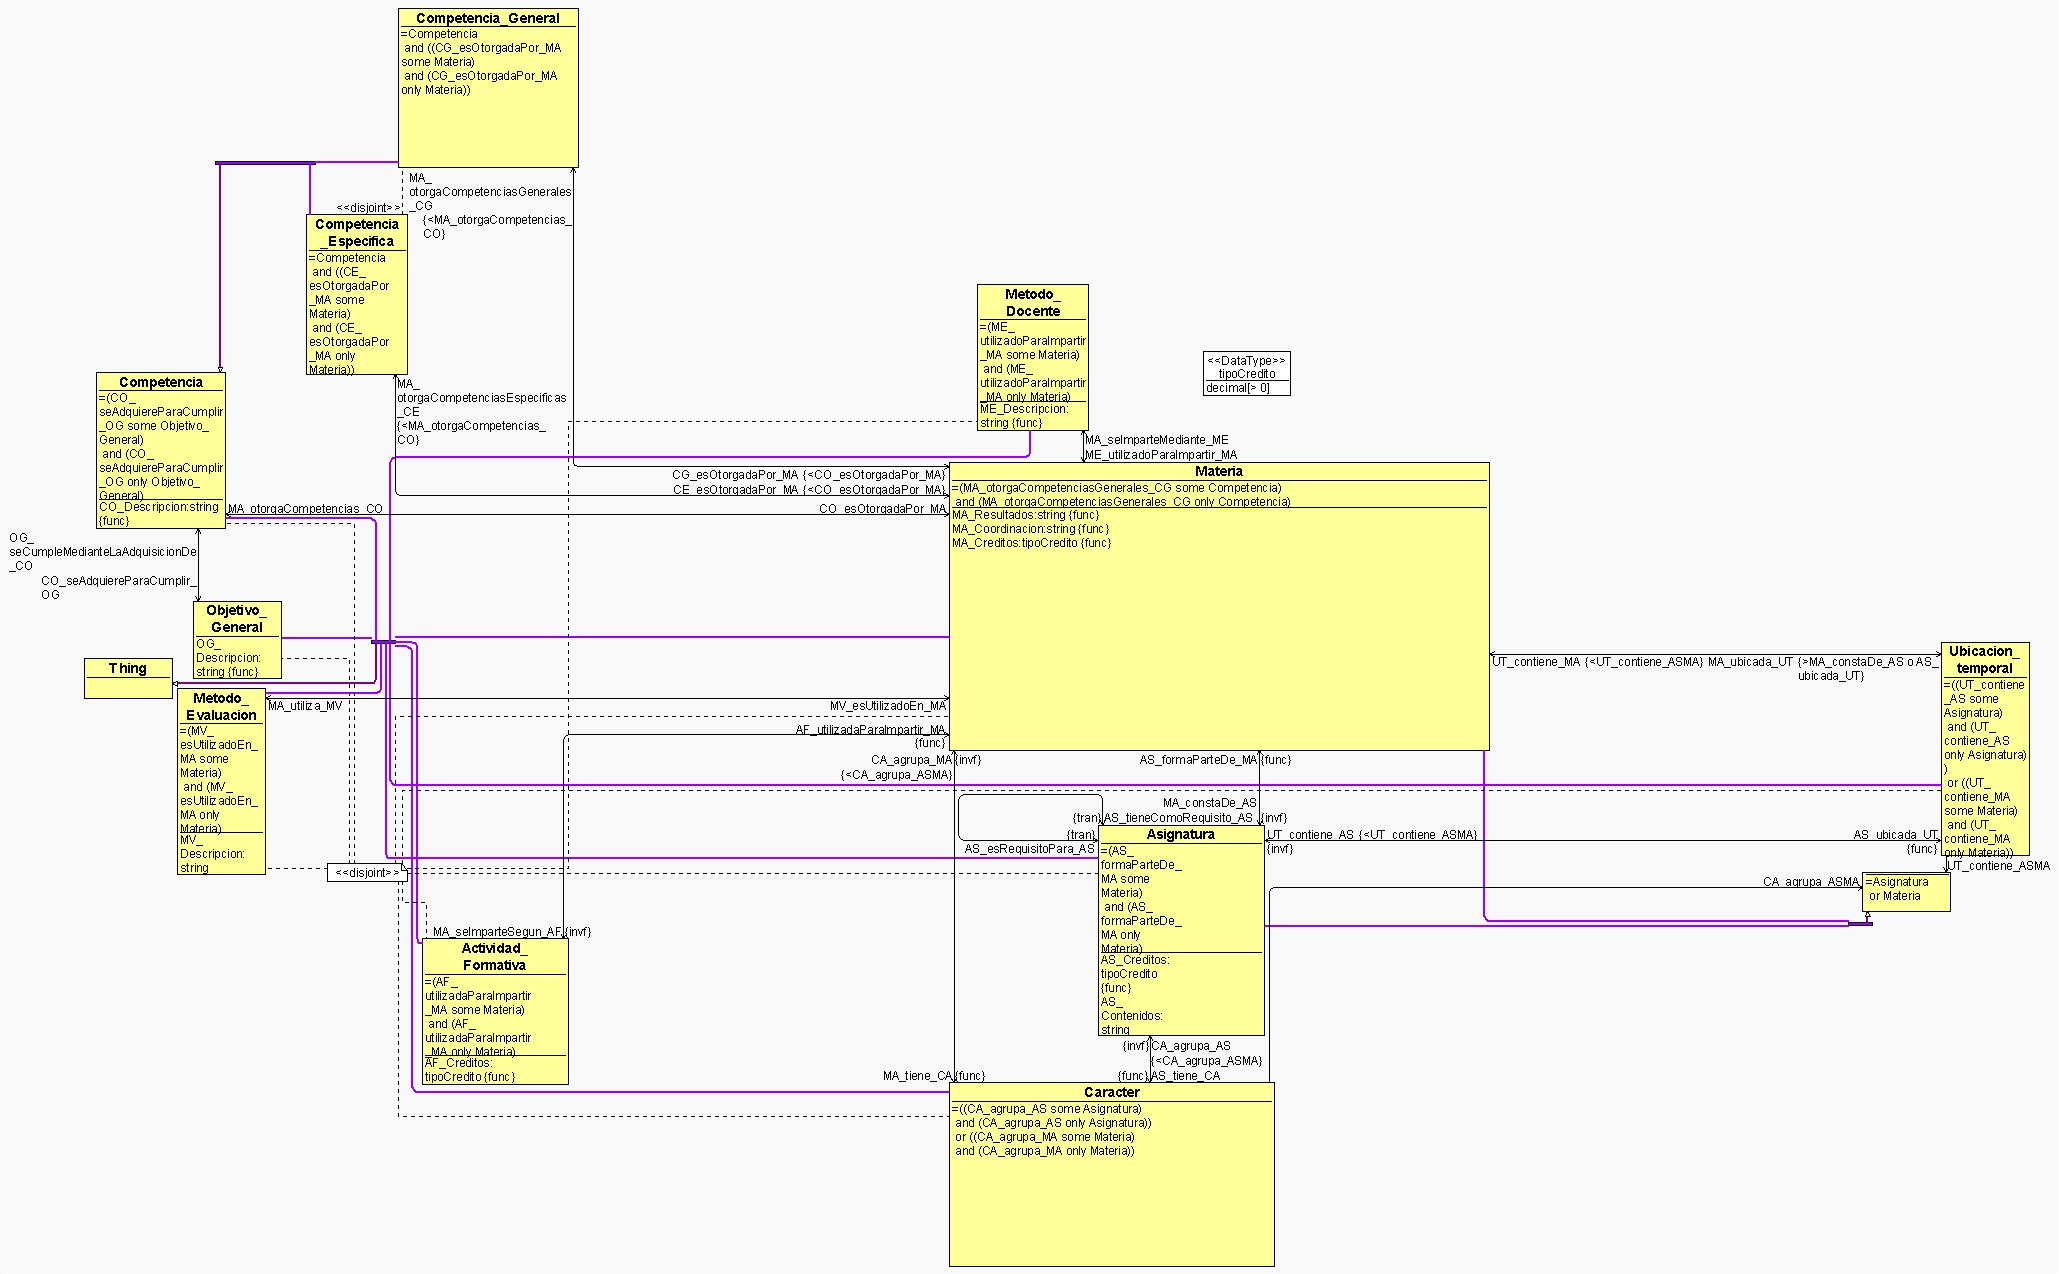
\includegraphics[width=1.00\textwidth]{Imagenes/Herramientas-OWLGrEd.png}
\end{center}

\subsubsection{SOVA} SOVA es un plugin de Protégé que permite la visualización de ontologías al completo. Gracias a SOVA, podemos tener en un mismo esquema clases, individuos y relaciones. 
SOVA tiene dos modos de trabajo. En el primer modo podemos ver la información tal y como está especificada en el fichero OWL. En el segundo modo la herramienta nos presenta una visión del fichero jerarquizada, pero con la limitación de sólo poder comprobar las relaciones entre individuos y clases, sin poder llegar a más detalle.

\todo{Captura realizada antes de la unión de abox y tbox}

\begin{center}
		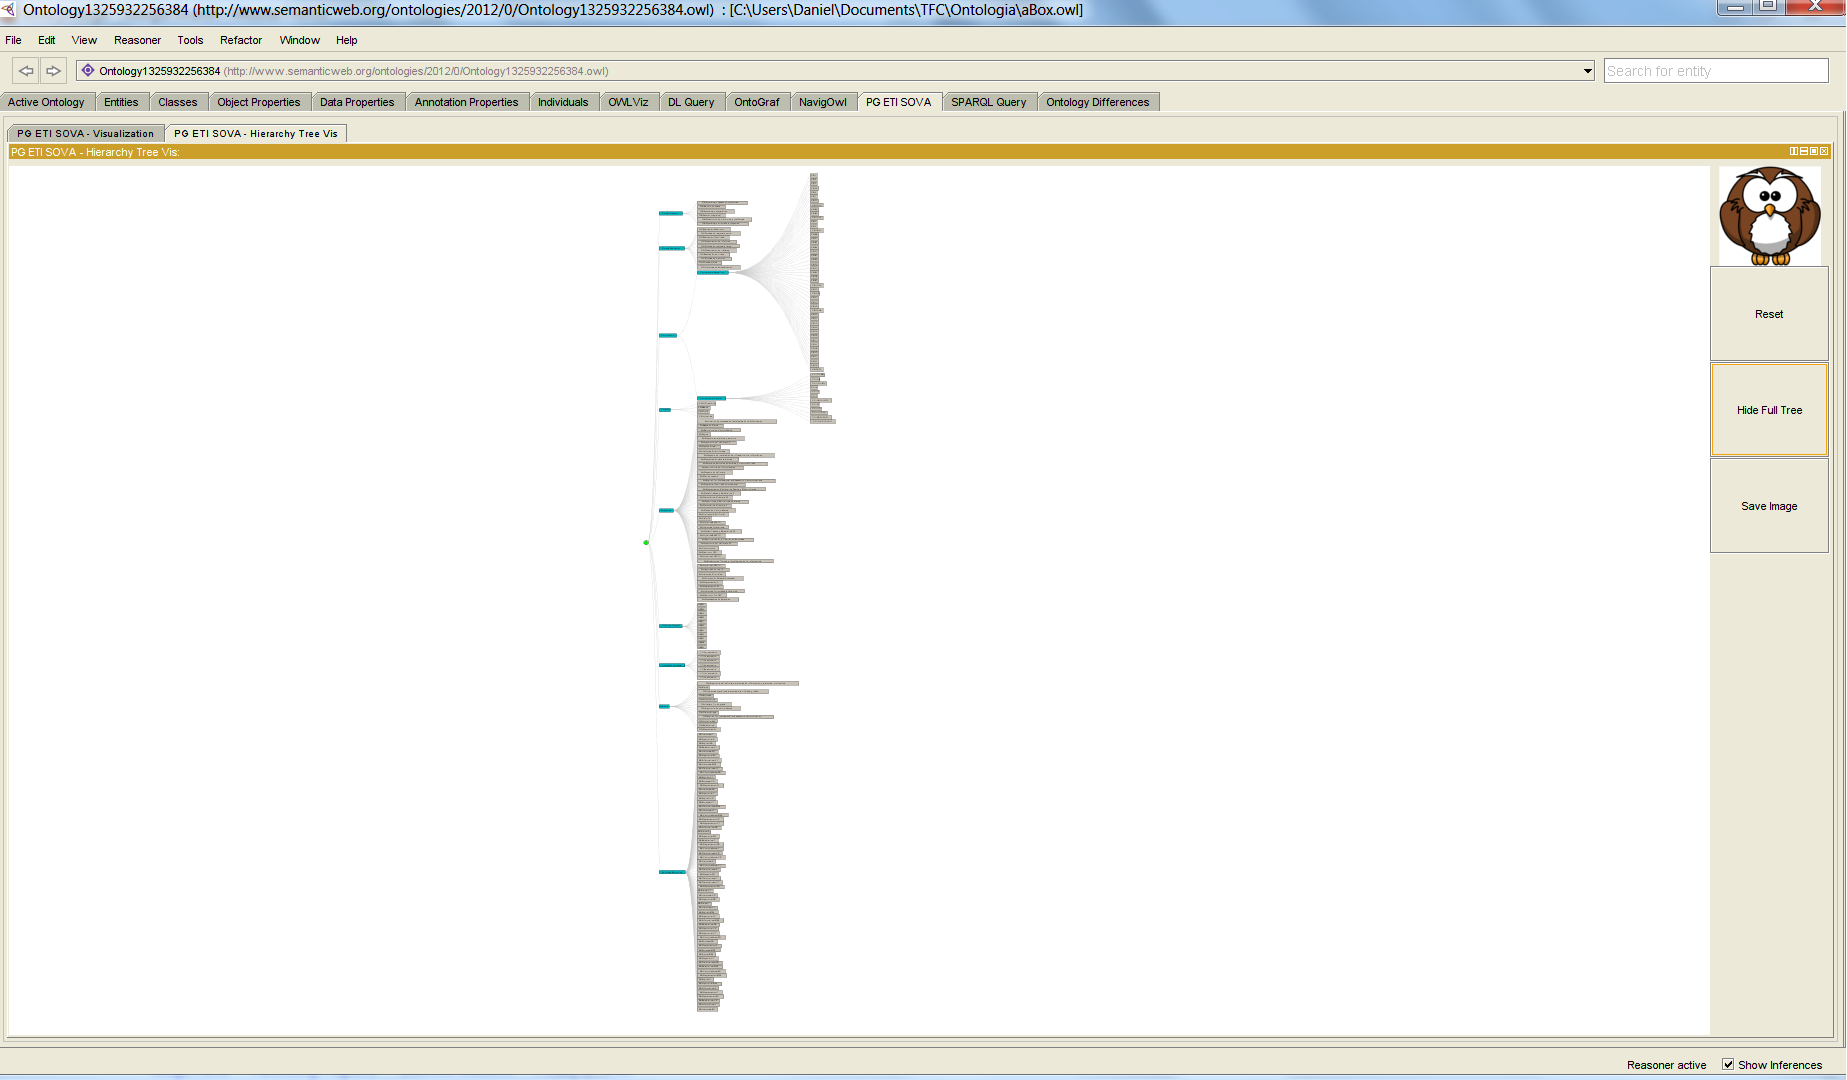
\includegraphics[width=1.00\textwidth]{Imagenes/Herramientas-SOVAhie.png}
\end{center}
\begin{center}
		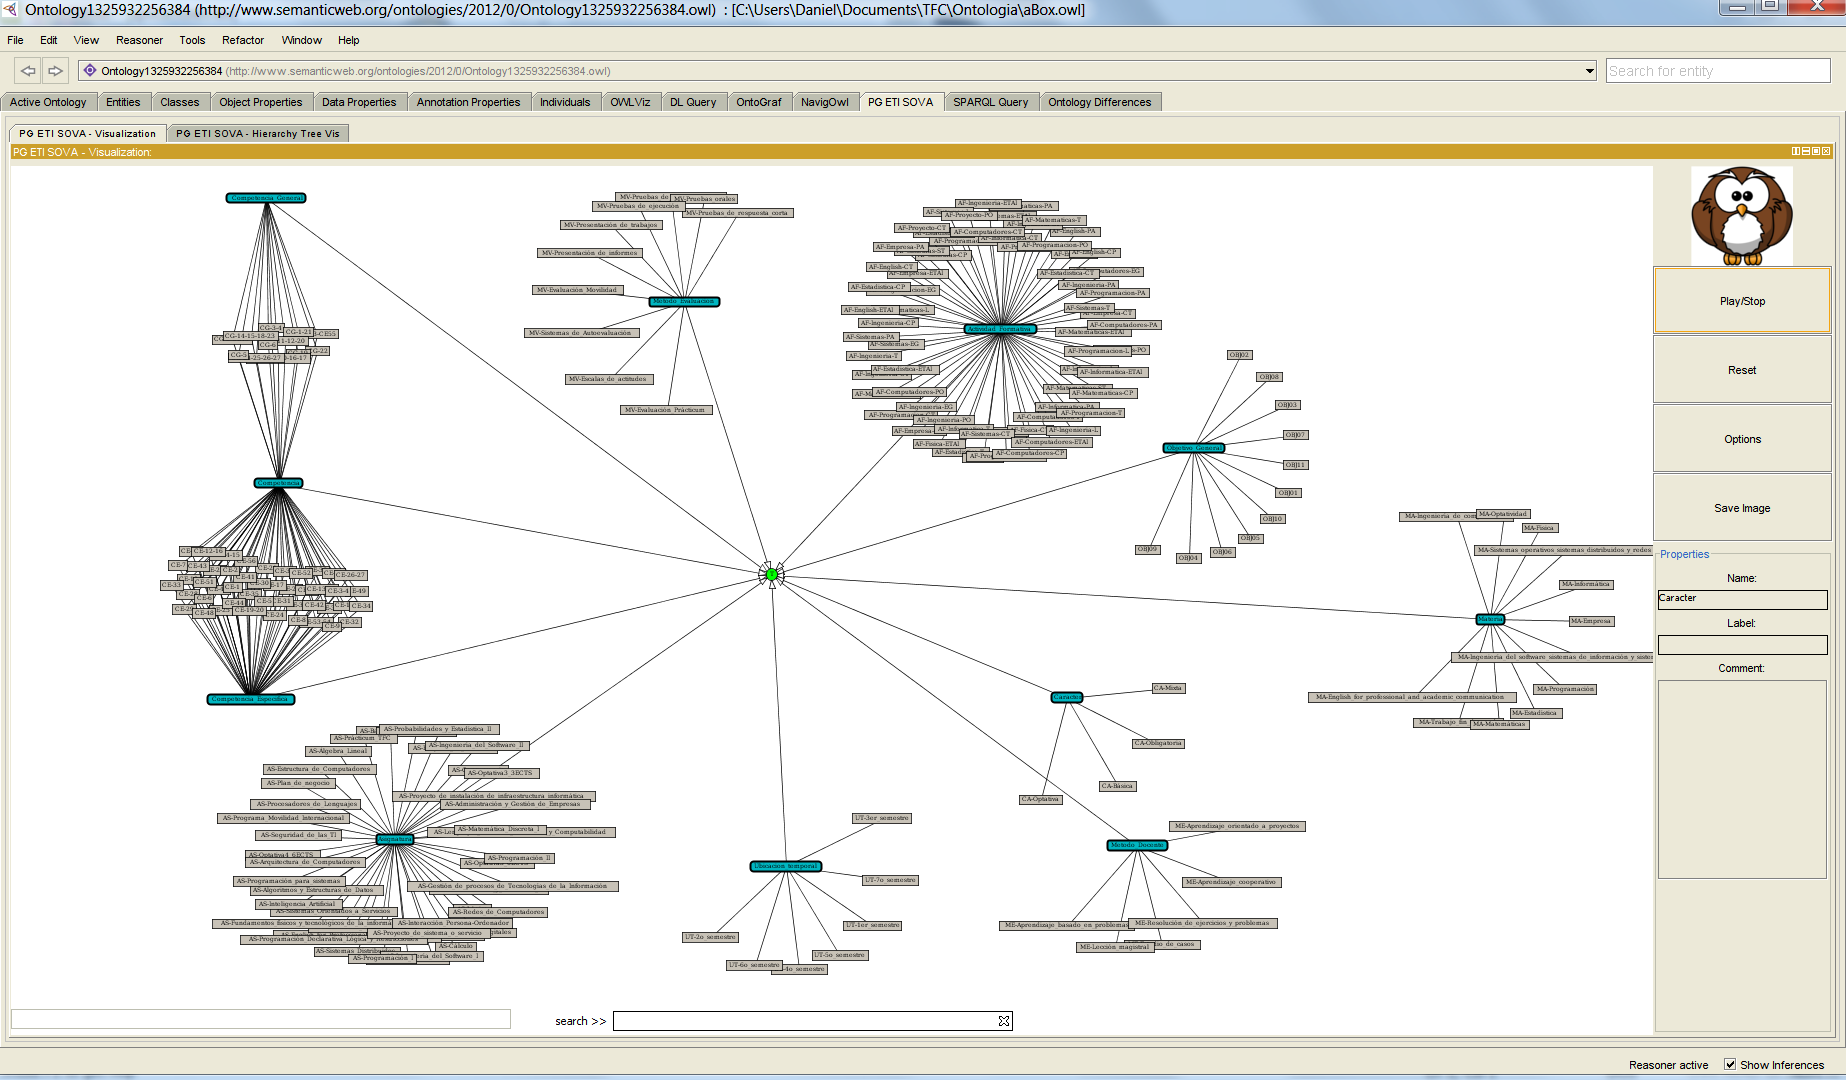
\includegraphics[width=1.00\textwidth]{Imagenes/Herramientas-SOVAvis.png}
\end{center}


\subsubsection{DL-Query}. Se trata de un plugin de Protégé que nos permite, mediante el uso de un razonador, realizar preguntas al razonador, utilizando para ello sintaxis Manchester. DL-QUery es capaz de contestar preguntas sobre cualquier aspecto de la ontología. 

Además, permite que una consulta que ea realizada a menudo, sea almacenada en la ontología como una clase definida, o bien como una clase anónima. Si el usuario de la ontología está familiariazado con la sintaxis Manchester, o bien incluimos las consultas a realizar a la ontología como clases definidas, dotaremos al usuario de las herramientas precisas para poder realizar preguntas sobre la ontología que lleven a un mejor diseño de la ontología.

\todo{Captura realizada antes de la unión de abox y tbox}

\begin{center}
		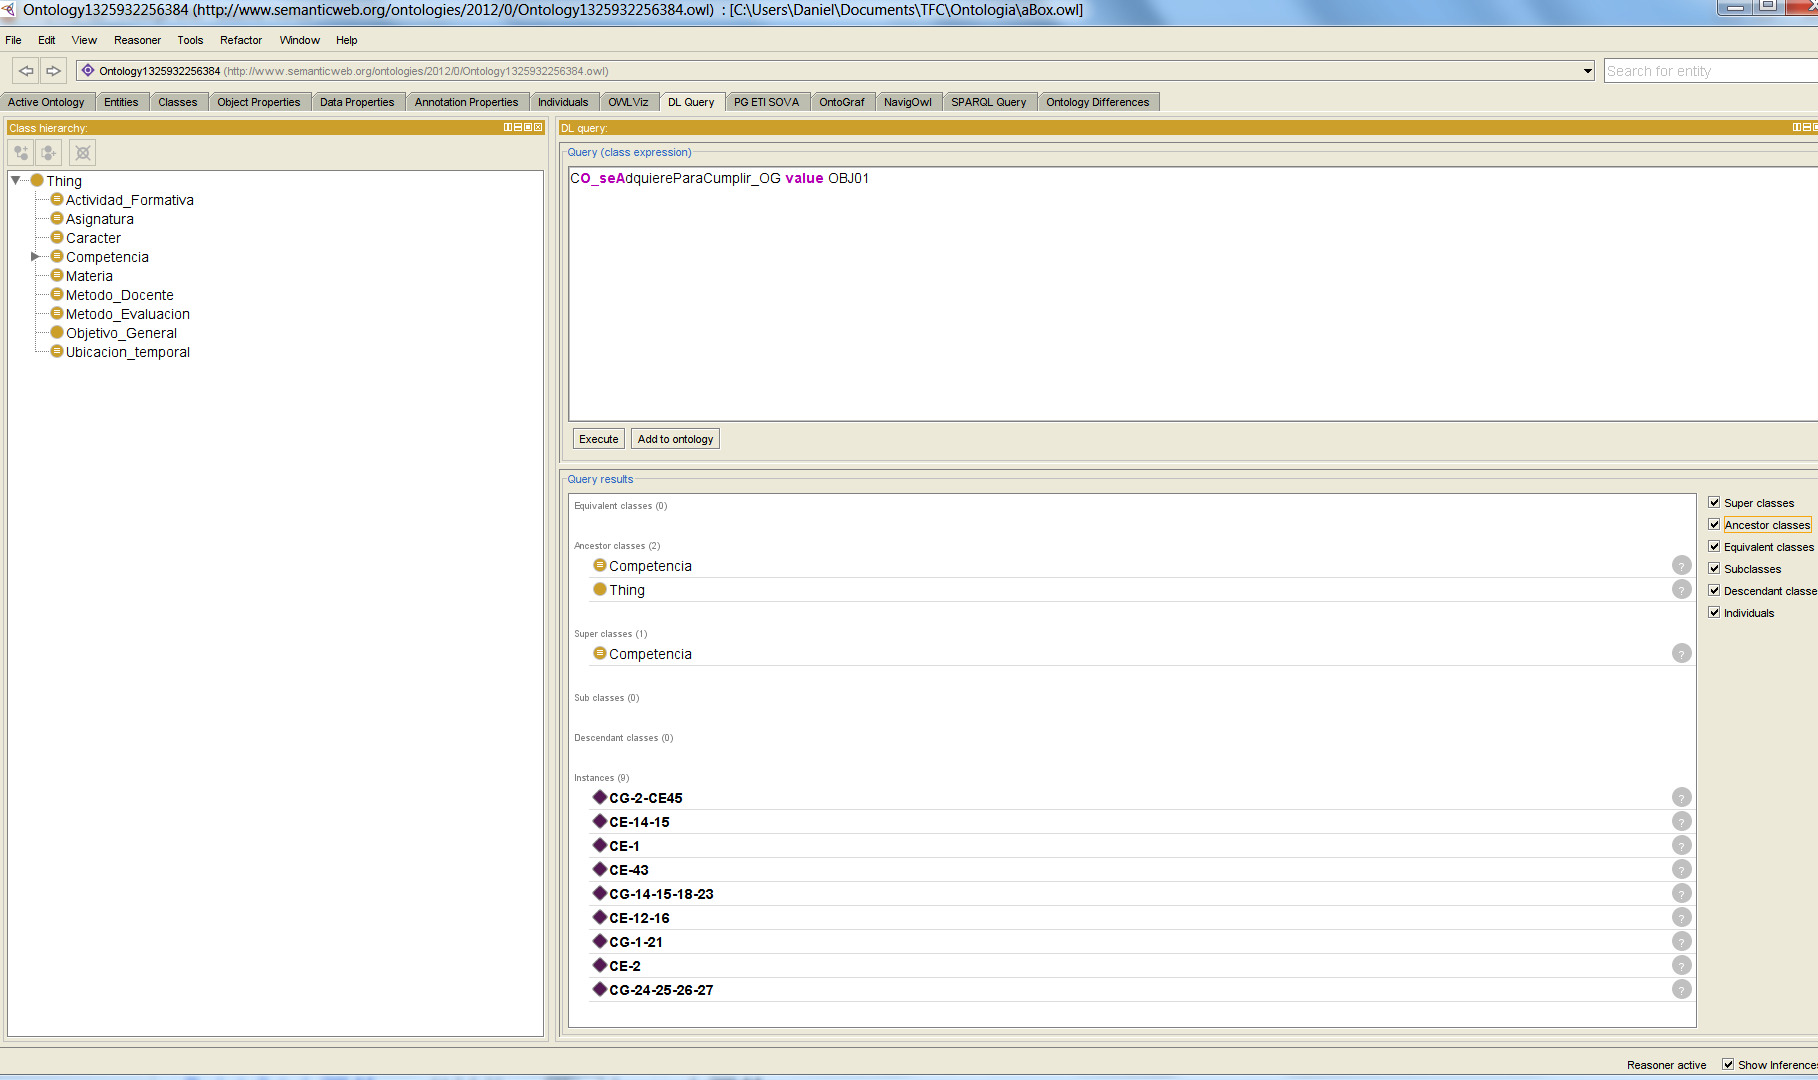
\includegraphics[width=1.00\textwidth]{Imagenes/Herramientas-DLQuery1.png}
\end{center}
\begin{center}
		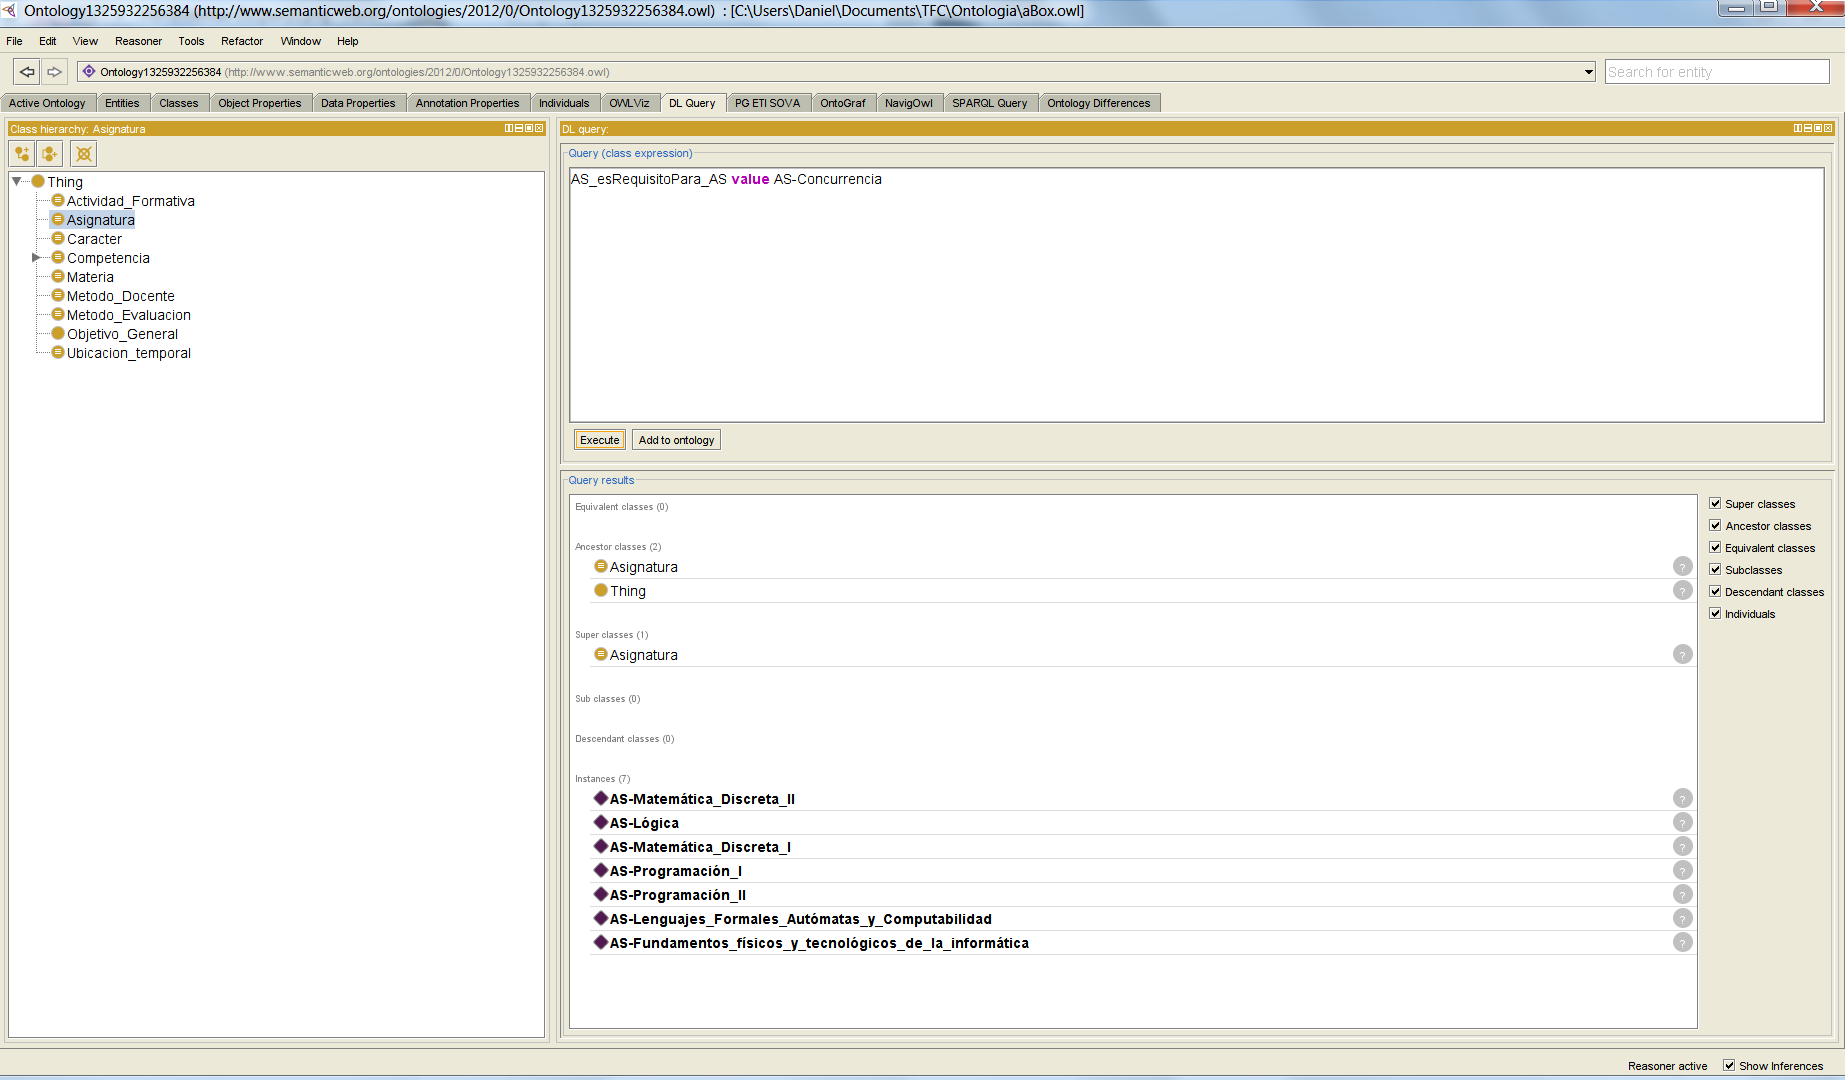
\includegraphics[width=1.00\textwidth]{Imagenes/Herramientas-DLQuery2.png}
\end{center}

\subsubsection{Cardinality View} Es un plugin, integrado en Protégé que nos permite visualizar las restricciones de cardinalidad de un modo mas amigable, sobre todo para personas no familiarizadas con la informática. Desde el mismo se pueden incluso editar dichas restricciones, añadir unas nuevas, o eliminar las ya existentes. Admite restricciones sobre clases, propiedades de datos, constantes de propiedades de datos e incluso de individuos.

\begin{center}
		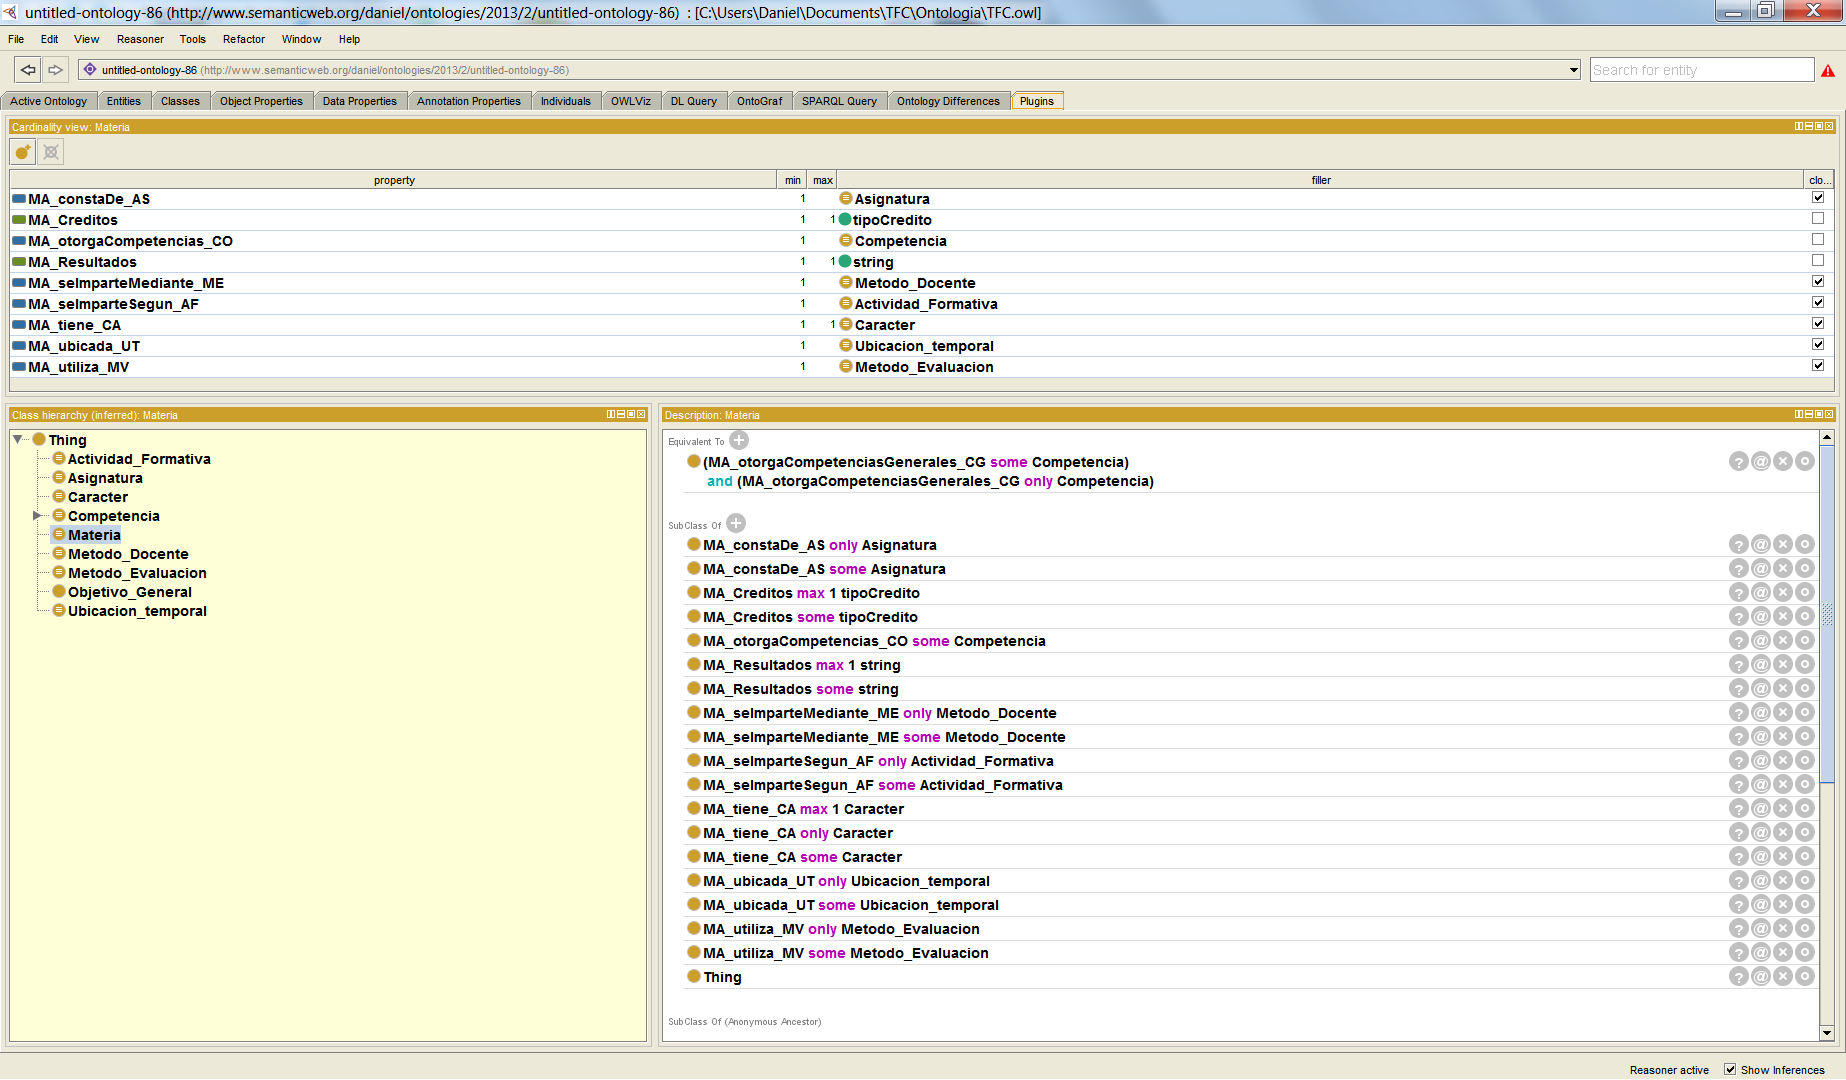
\includegraphics[width=1.00\textwidth]{Imagenes/Herramientas-CardinalityView.png}
\end{center}

\subsubsection{Outline and Existential Tree Views} nos permite visualizar las relaciones existenciales de la ontología en forma de arbol, a partir de cualquier nodo, y pudiendo colgar en él las propiedades de objetos y datos. De este modo, podemos obtener una visión de la ontología desde la parte dela misma que en cada momento nos resulte de interés, facilitando la comprensión y el acceso a la información.

\begin{center}
		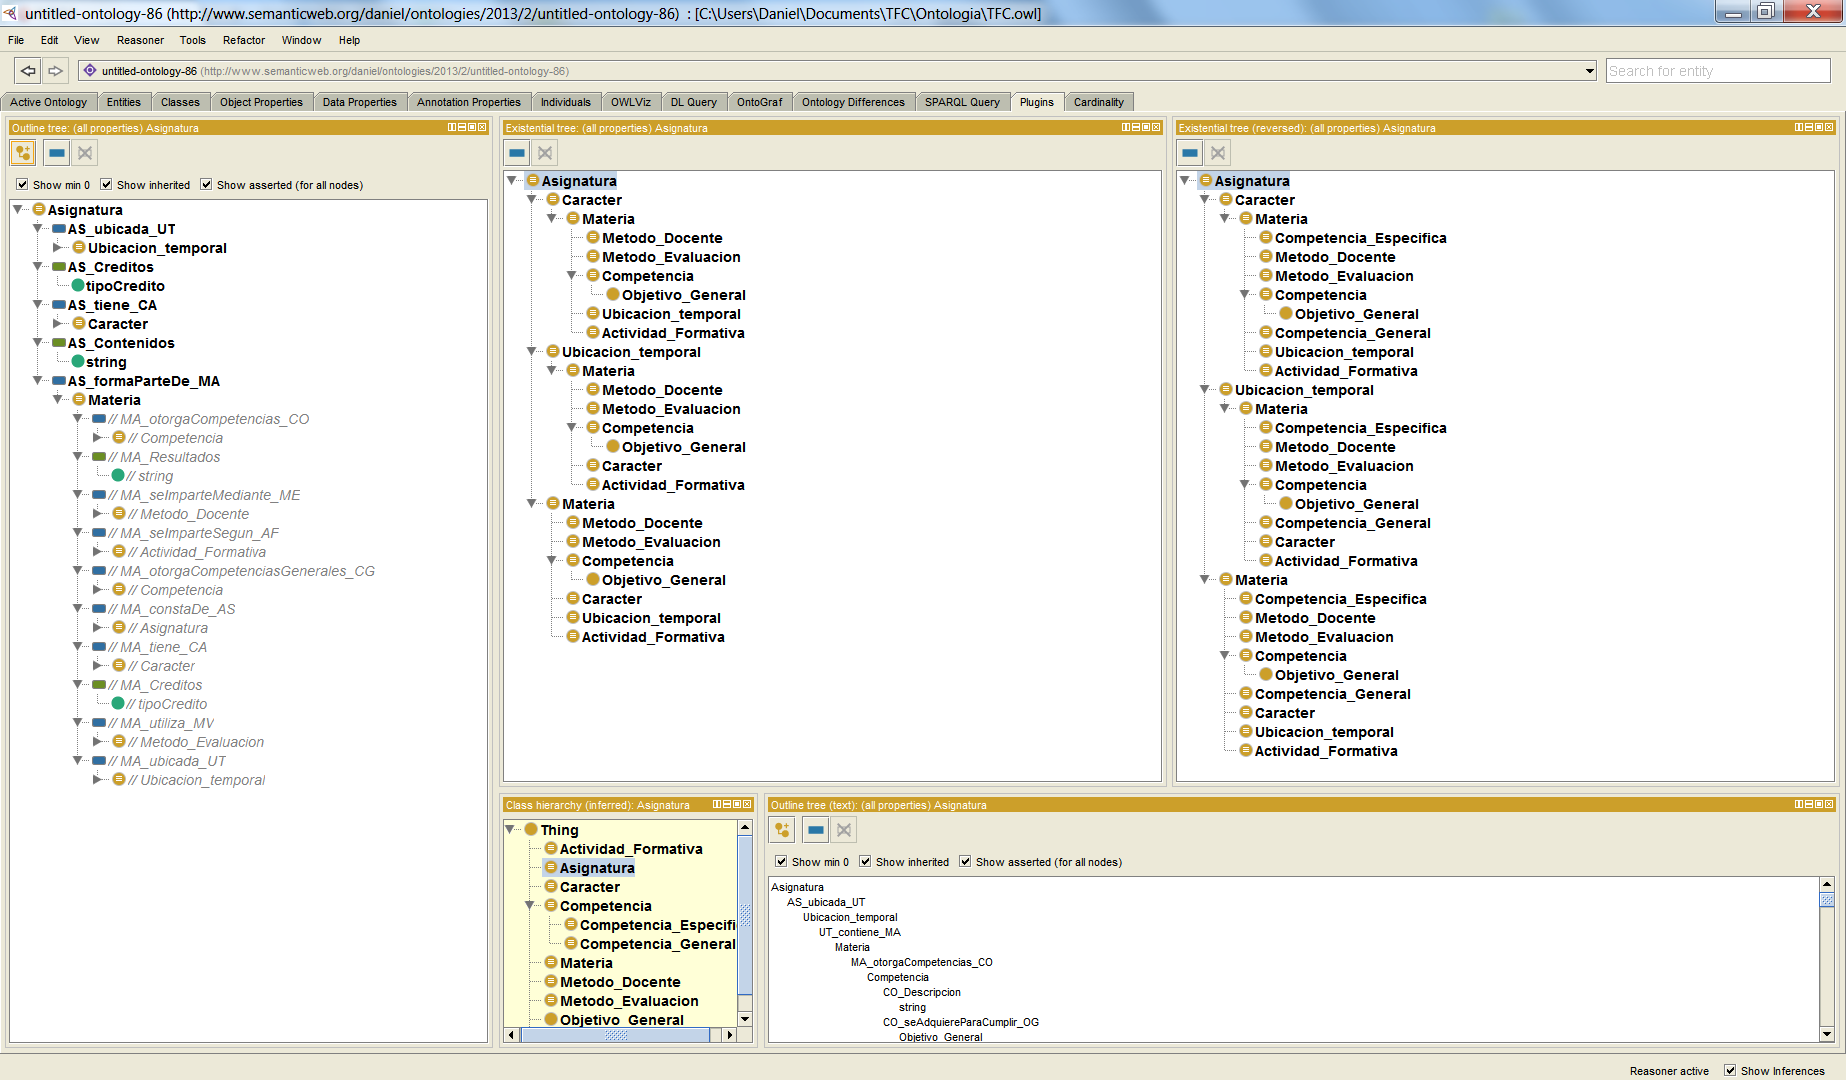
\includegraphics[width=1.00\textwidth]{Imagenes/Herramientas-ExistentialTree.png}
\end{center}

\subsubsection{OWLDoc} es un plugin de Protégé que permite exportar la información contenida en la ontología a HTML, de modo que la visualización de la información puede sere más amena y flexible. OWLDoc exporta toda la información. En la documentación que genera encontramos todo lo relativo a clases, propiedades sobre objetos, propiedades sobre datos, y además, sobre los individuos de la ontología e incluso sobre los tipos de datos que hemos utilizado en la misma.

\begin{center}
		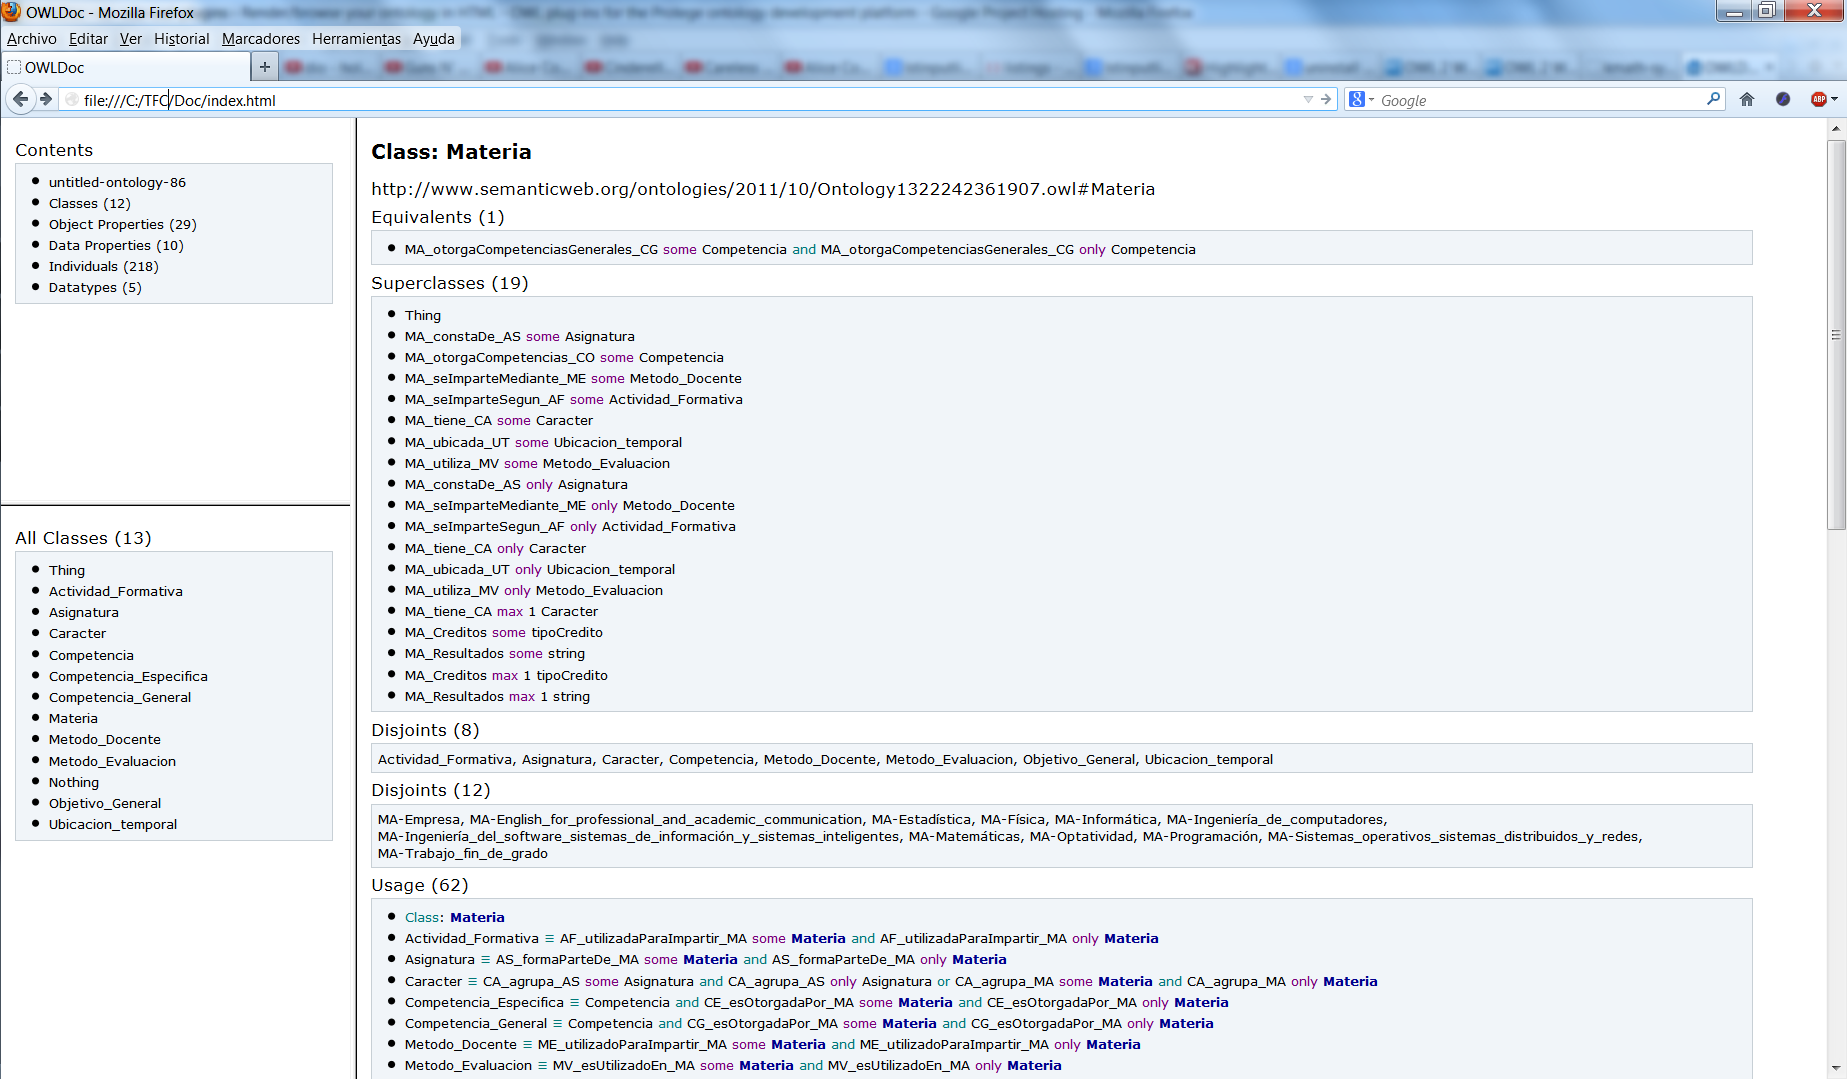
\includegraphics[width=1.00\textwidth]{Imagenes/Herramientas-OWLDoc.png}
\end{center}

\subsubsection{OWLViz} Plugin de Protégé, muy básico, que permite navegar únicamente sobre las clases de la ontología. No permite acceder a información contenida en las clases, o a las relaciones entre ellas, limitándose´a mostrar relaciones del tipo "es un". 

\subsubsection{OWLPropViz} Plugin basado en OWLViz, que además de mostrar relaciones del tipo "es-un", nos enseña relaciones de equivalencia, clases disjuntas, y otras propiedades sobre objetos definidas en la ontología. 
Por desgracia, no he sido capaz de lograr que funcione. El plugin figura como compatible únicamente con la versión 4.0 de Protégé, y no se ha logrado que funcione en versiones superiores como 4.1 y 4.2 rc1. Para más inri, no se encuentra la versión 4.0 de Protégé disponible para la descarga, por lo que no podemos comprobar la verdadera utilidad de este plugin.

\subsubsection{OWLDiff} Herramienta disponible para uso denteo de Protégé en forma de plugin o como un programa individual que nos permite comparar dos ontologías, mostrándonos las diferencias y similitudes entre ellas, unirlas en una única ontología, y realizar inferencias sobre ellas utilizando el razonador Pellet. Podemos ver el resultado de la comparativa en forma de axiomas o inserciones de la ontología y cada uno de ellos en sintaxis DL o Manchester.
Además tiene la posibilidad de integrarse en varios sistemas de control de versiones, como Subversion, lo que facilita el trabajo sobre la ontología por un amplio grupo de gente.

\begin{center}
		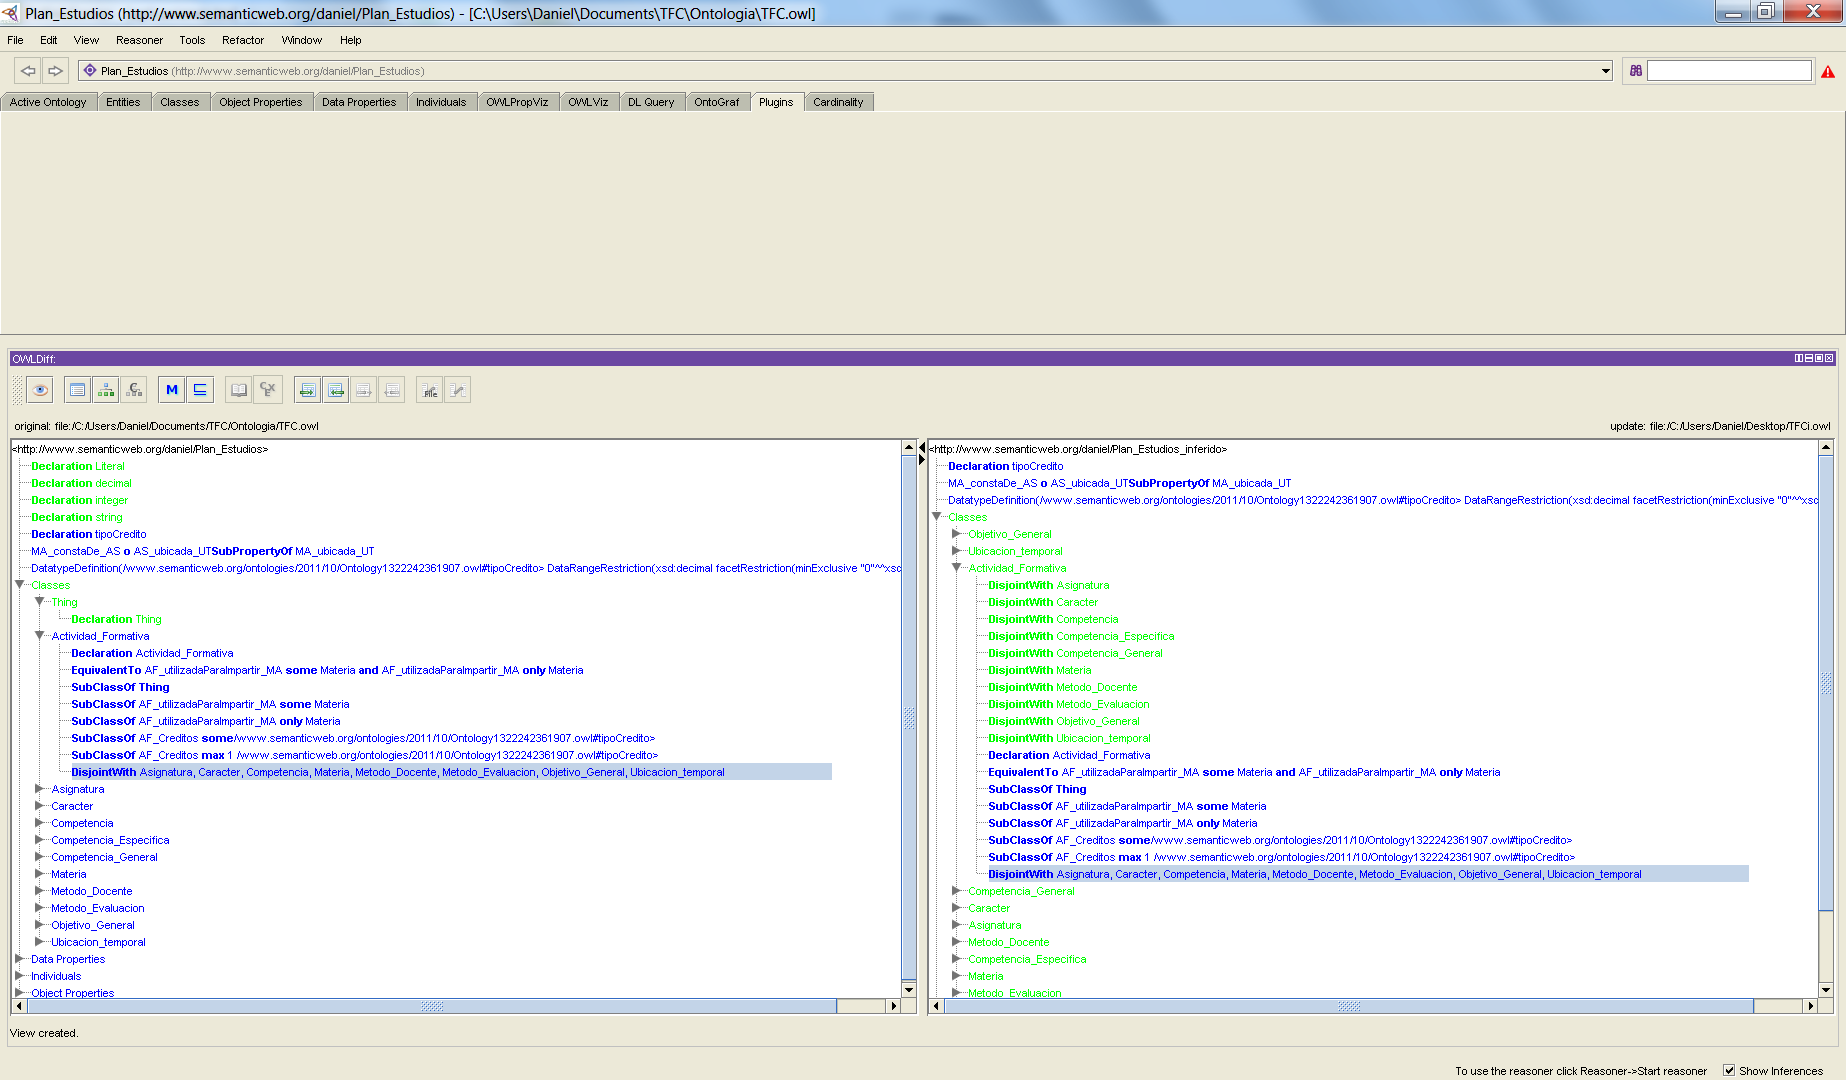
\includegraphics[width=1.00\textwidth]{Imagenes/Herramientas-OWLdiff.png}
\end{center}


\subsection{Transformación de datos}

\subsubsection{OWL2RDB} es un plugin para Protégé que permite transformar ontologías OWL2 en bases de datos relacionales. Por desgracia, el plugin no funciona correctamente con versiones actuales de java y no se distribuye ningún tipo de documentación ni existe página web del autor u otras donde se mencione la aplicación, a donde podamos dirigirnos para obtener más información acerca del error. Nos parecía muy interesante el poder exportar la ontología a una base de datos y trabajar con herramientas especializadas sobre ella.

\subsection{Otros}

\subsubsection{AceWIKI}. Potente herramienta que nos permite construir una wiki semántica utilizando el lenguaje ACE, lo que permite que cualquier usuario, sin tener que lidiar con RDF o OWL, pueda construir y mantener el wiki, además manteniendo siempre la coherencia del contenido. 

Si bien resulta perfecta para crear cualquier ontología desde cero utilizando únicamente el lenguaje natural, no es posible la creación de una wiki desde una ontología dada, ya que las los individuos, clases y propiedades están contenidas en el propio artículo, y no en anotaciones sobre la ontología, como en otros constructores.

http://attempto.ifi.uzh.ch/acewiki/

\subsubsection{Wikis Semánticas} Las wikis semánticas permiten incorporar a una wiki ordinaria, un modelo de datos que permite capturar e identificar relaciones entre los diversos conceptos, de modo que es posible realizar consutas sobre el contenido y sus relaciones.

	El software de wiki semántica más extendido son Freebase, OntoWiki y Semantic Media Wiki.
	
	Freebase consta de una colección de datos estrucutrados en linea, obtenidos a partir de muy diversas fuentes, con el objetivo de crear un recurso global online que permite a los usuarios un acceso a la información eficaz y equitativo. Metaweb fue adquirida por Google en 2010. Un usuario puede realizar aportaciones a freebase, pero el esquema de datos de su aportación no se adapta al común de la aplicación hasta que un empleado de la compañia le da su visto bueno. 
	
	OntoWiki es una herramienta que permite la visualización de la infromación contenida en en una base del conocimiento, con varios puntos de vista sobre cada dato. permite la edición de la información de un modo simple,  y la discusión acerca de cada cambio realizado gracias a su control de cambios. 
	
	Semantic MediaWiki es una extensión de MediaWiki (herramienta para la realización de wikis sintácticas) que permite transformar una wiki sintáctica en una wiki semántica. La principal ventaja de de SMW es la cantidad de extensiones disponibles para personalizar la wiki y añadir nuevas utilidades.
	
	La principal ventaja de SMW sobre MediaWiki sobre los otros gestores de wikis es la cantidad de funcionalidades que, en forma de añadido, se pueden utilizar para ampliar las capacidades de las wikis creadas.
	
	A modo de ejemplo, se ha construido una wiki con la ontología del ejemplo. Como inconveniente destacamos el hecho de que algunas estructuras semánticas no se puedan incorporar a la wiki (como una limitación en el número - al menos una- de asinaturas que componen una materia), la imposibilidad de utilizar un razonador directamente sobre la misma, y las actuaciones sobre la ontología deben ser luego trasladadas a mano sobre la wiki, ya que por el momento no se ha encontrado una herramienta que realice este trasvase de información de manera automática \footnote{las limitaciones sobre las estructuras semánticas soportadas por la wiki, hace que en ontologías complejas como la que estamos abordando existan construcciones que no son traducibles directamente a la wiki}, al menos con las herramientas encontradas en el directorio de extensiones de MediaWiki y Semantic MediaWiki.
	
	Como punto a su favor, las wikis son extremadamente fáciles de crear y mantener, y además, cuentan con extensiones que facilitan la interacción con el usuario y protegen a la wiki de cambios que destruyan la coherencia de la información almacenada.
	
	\paragraph{Puesta en marcha de la wiki}
	Para poner en marcha la wiki, es preciso instalar un servidor web, php y un gestor de bases de datos. En la wiki creada al efecto hemos utilizado el software apache 2.2.22, php 5.4.6-1 y mysql 5.5.29. Sobre ello hemos puesto en marcha la versión 1.20 de Mediawiki y hemos instalado las extensiones SemanticMediaWiki 1.8 y Semantic Forms 2.1 para crear formularios para la introducción de la información por parte de los usuarios y disminuir, si no evitar, errores semánticos. Adicionalmente se recomienda permitir la edición de artículos únicamente a los usuarios editores y administradores.
	
	Se han probado varias extensiones de Mediawiki y SMW que permiten subir una ontología en formato RDF/XML a la wiki, como Ontology Editor o RDFIO, pero dada la complejidad de la ontología, muchas de las restricciones impuestas causaban que la extensión fallase, o en el mejor de los casos, simplemente ignorasen esas restricciones, provocando comportamientos no deseados en la ontología. Finalmente, se ha optado por crear la wiki de forma manual, al no contar con herramientas fiables que permitan el volcado de información de forma fiable, y con el fin de poder mostrar la idoneidad de trabajar con herramientas semánticas, como ontologías y wikis semánticas, cuando se trata de proyectos o trabajo cuyo principal objetivo es el de capturar conocimiento.
	
	\todo{Adjuntar algunas capturas de pantalla de la wiki en el documento}



%\todo{Consideramos SPARQL útil? par apoder utilizarlo}
%\todo{las otras herramientas como tabajo a futro/mejoras}

%%% Local Variables: 
%%% mode: latex
%%% TeX-master: "tfc-ontologia-grado"
%%% TeX-PDF-mode: t
%%% ispell-local-dictionary: "castellano"
%%% End: 
